%%%%%%%%%%%%%%%%%%%%%%%%%%%%%%%%%%%%%%%%%%%%%%%%%%%%%%%%%%%%%%%%%%%%
% Grundlagen
%%%%%%%%%%%%%%%%%%%%%%%%%%%%%%%%%%%%%%%%%%%%%%%%%%%%%%%%%%%%%%%%%%%%

\chapter{Stand der Technik}
  \label{Stand der Technik}

\medskip
Bisher findet Navigation hauptsächlich im Freien statt. Zum Beispiel schon seit langem bei Navigationssystemen für Autos. Dabei wird ausschließlich GPS verwendet. Für Navigation innerhalb von Gebäuden ist GPS nicht brauchbar. Es ist zu ungenau und wird durch die Wände des Gebäudes noch zusätzlich ungenauer. Bei der genauen positionsbestimmung wird es zunehmend wichtiger auch die Orientierung zu bestimmen. Denn innerhalb von Gebäuden und bei Positionsunterschieden von wenigen Metern ist die Information in welche Richtung man schaut ebenfalls interessant und liefert zusätzliche Information. Gerade bei einer Navigations-App für Bibliotheken ist es wichtig zu wissen welches Regal gerade angeschaut wird. Außerdem darf die Position eine Ungenauigkeit von einigen Zentimetern nicht überschreiten, denn sonst ist die Führung zum Buch so ungenau, dass die App mehr Umstand als Nutzen bringt.

\section{Beschreibung der Orientierung von Objekten im dreidimensionalen Raum}
Zur Beschreibung der Orientierung von Objekten im dreidimensionalen Raum in kartesischen Koordinatensystemen gibt es mehrere Möglichkeiten. Die drei am häufigsten verwendeten und für uns relevanten werden im Folgenden vorgestellt.

\subsection{Euler-Winkel}
Bei Euler-Winkeln handelt es sich um drei Winkel die jeweils die Rotation um eine bestimmte Achse des Koordinatensystems angeben. So kann eine Transformation zwischen zwei Koordinatensystemen, dem Labor- und dem Körperfesten-System definiert werden.

Es existieren mehrere Definitionen von Euler-Winkeln, was die Reihenfolge der Drehungen um die Achsen anbelangt. Für unsere Zwecke beschäftigen wir uns mit Yaw-Pitch-Roll - zu deutsch: Roll-Nick-Gier-Winkel. Dies entspricht auch der Luftfahrtnorm (DIN 9300).


\begin{itemize}
	\item Roll (Roll-Winkel) beschreibt die Querneigung, also die Drehung um die X-Achse.
	\item Pitch (Nick-Winkel) besschreibt die Längsneigung, also die Drehung um die Y-Achse.
	\item Yaw (Gier-Winkel) beschreibt Orientierung, also die Drehung um die Z-Achse.
\end{itemize}

Bei mobilen Geräten wie dem Apple iPhone gibt es anders als bei Fahrzeugen keine fest denifierte Ausrichtung. Beim iPhone und iPad sind die Winkel darum so verteilt wie auf Bild \ref{fig:apple-axes} zu sehen.

\begin{figure}[htb]
\centering
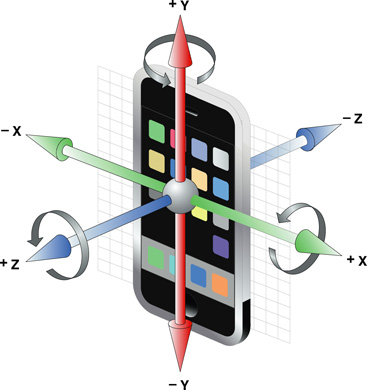
\includegraphics[scale=0.8]{figures/apple-axes}
\caption{Roll-Pitch-Yaw \cite{apple:001}}
\label{fig:apple-axes}
\end{figure}

Euler-Winkel habend en Vorteil, dass sie jeder intuitiv verstehen kann. Somit kann man mit ihnen auch einfach rechnen.

\textcolor{red}{Nachteil Gimbal-Lock.}

\subsection{Rotationsmatrizen}
Eine Rotationsmatrix ist eine orthogonale Matrix, die ebenfalls die Drehung im Raum beschreibt.

Kein Vorteil zu Euler-Winkeln, Gimbal-Lock auch vorhanden. Kompliziert zu rechnen.

\subsection{Quaternionen}
Vorteil: Kein Gimbal-Lock
Nachteil: Kompliziert zu rechnen.

\section{Positionsbestimmung}
Die Positionsbestimmung erfolgt in unserem Fall über Bluetoo